\documentclass[class=report, crop=false, 12pt,a4paper]{standalone}
\usepackage{enumitem}
\usepackage{float}
\usepackage[normalem]{ulem}
\usepackage{graphicx}
\usepackage{amsmath}
\usepackage{amssymb}
\usepackage{siunitx}
\usepackage{commath}
\usepackage{tikz}
\usetikzlibrary{positioning, fit, calc}   
\tikzset{block/.style={draw, thick, text width=3cm ,minimum height=1.3cm, align=center},   
line/.style={-latex}     
}  
\begin{document}
\section{Tutorial Week 1: Continuity Equation}
\subsection{Exercise 2}
\subsubsection{Is the system steady?}
The system is steady due to the fact that our velocity field has no terms in $t$, meaning that our flow does not change with time - steady flow.
\subsubsection{Is the fluid incompressible?}
If fluid is incompressible $\nabla \cdot\vec{V} = 0$
\begin{gather}
  \frac{\partial v}{\partial y} = \frac{4}{y} -2\\
  \therefore \nabla \cdot \vec{V} = \frac{4}{y} - 2 \neq 0
\end{gather}
Hence, fluid is compressible.
\subsubsection{Make a vector map of the velocity field}
Using the following code, a vector field was mapped.
\begin{verbatim}
  %Hasha Dar
  clc
  clear
  close all
  
  [x,y]=meshgrid(-2:0.5:2,1:0.5:4); %field
  
  u = 0.*x; %x vector
  v = (4.*log(y) -2.*y + 10); %y vector
  
  quiver(x, y, u, v) %plots quiver with arrow base at x, y 
  and direction u, v
  axis([-2.5 2.5 0.5 5]) %formatting
\end{verbatim}
This produced the following plot:
\begin{figure}[H]
  \centering
  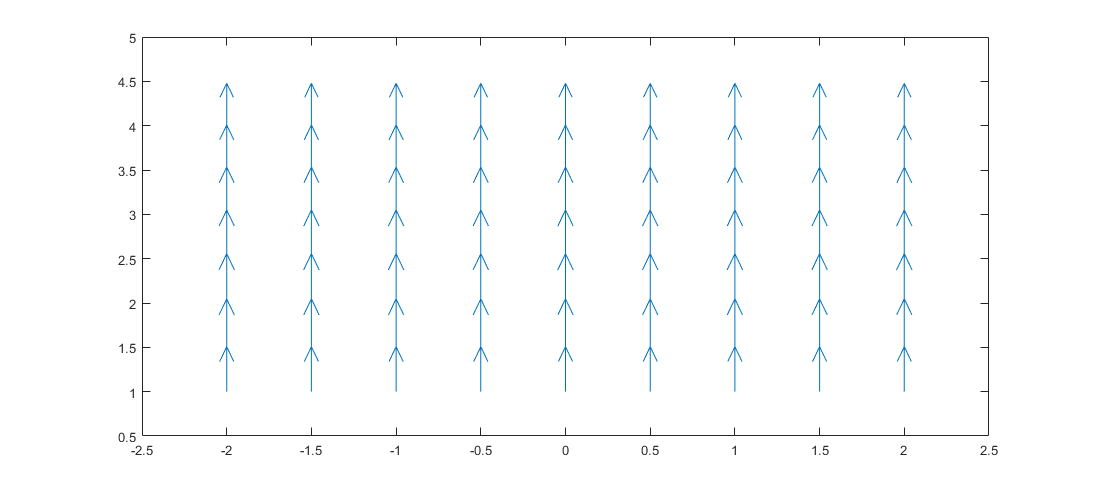
\includegraphics[width = \textwidth]{../img/quiverplotexercise20011-002.png}
\end{figure}
\subsubsection{Determine the variation of the volume dilatation rate in the flow domain}
\begin{gather}
  v = 4\ln{y} - 2y + 10\\
  \textrm{Volume dilatation rate} \rightarrow \frac{\partial v}{\partial y} = \frac{4}{y} - 2\\
\end{gather}
For the range $1 < y < 4$, the variation in the volume dilatation is negative, hence our fluid is compressible. 
\subsubsection{Estimate the volume dilatation rate in points $(0, \ 1)$ and $(0, \ 3)$ of the flow domain}
\begin{gather}
  (0, \ 1) \rightarrow \frac{4}{1} - 2 = 2 \ \si{\per\second}\\
  (0, \ 3) \rightarrow \frac{4}{3} - 2 = -\frac{2}{3} \ \si{\per\second}
\end{gather}
\subsubsection{Sketch how a squared fluid parcel located in the points above would deform}
\begin{figure}
  \centering
  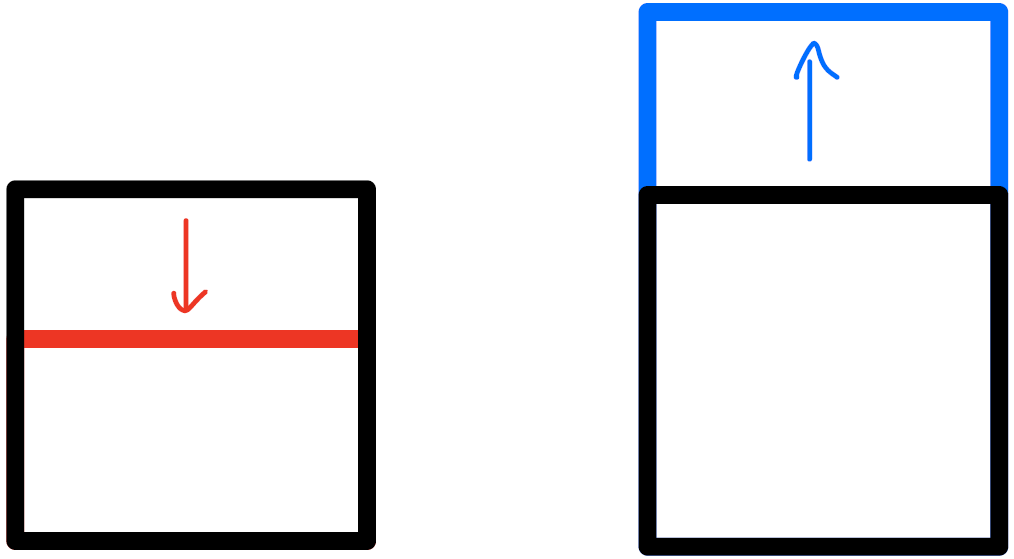
\includegraphics[width = 0.8 \textwidth]{../img/fluidparcelcompression.png}
  \caption{The right shows the fluid parcel being stretched vertically, due to the volume dilatation rate being positive at $(0, \ 1)$. The left shows the fluid parcel being compressed vertically, due to the volume dilatation rate being negative at $(0, \ 3)$}
\end{figure}
\subsubsection{Are there points in the flow domain which are not subject to a variation of the dilatation rate? Find their locus}
Points which are not subjected to volume dilatation rate are those that satisfy the condition $\nabla \cdot \vec{V}(x, \ y) = 0$
\begin{gather}
  \frac{4}{y}-2 = 0\\
  y = 2 \rightarrow (0, \ 2)
\end{gather}
\subsubsection{If the fluid is compressible determine how the density change in space (hint: assume $\rho$ is only a function of y). Estimate the density of point (0,2); comment your results}
Using continuity equation:
\begin{gather}
  \nabla \cdot (\rho \cdot \vec{V}) = \frac{\partial \rho u}{\partial x} + \frac{\partial \rho v}{\partial y} + \frac{\partial \rho w}{\partial z} \\
  \frac{\partial \rho(y) v(y)}{\partial y} = 0\\
  \rho(y)\cdot v(y) = A \textrm{ constant}\\
  \rho(y) = \frac{A}{4\ln{y} - 2y +10}\\
  \frac{A}{-2+10} = 1.2\\
  A = 9.6 \ \si{\kg\second\per\meter\squared}\\
  \rho(y) = \frac{9.6}{4\ln{2} - 2y +10} = 1.09 \ \si{\kg\per\meter\cubed} 
\end{gather}
\subsubsection{Make a contour map of the density and identify regions of compression and expansion. Are these in agreement with yours findings from the volume dilatation rate (you can use the contourf command in Matlab)?}
\begin{figure}[H]
  \centering
  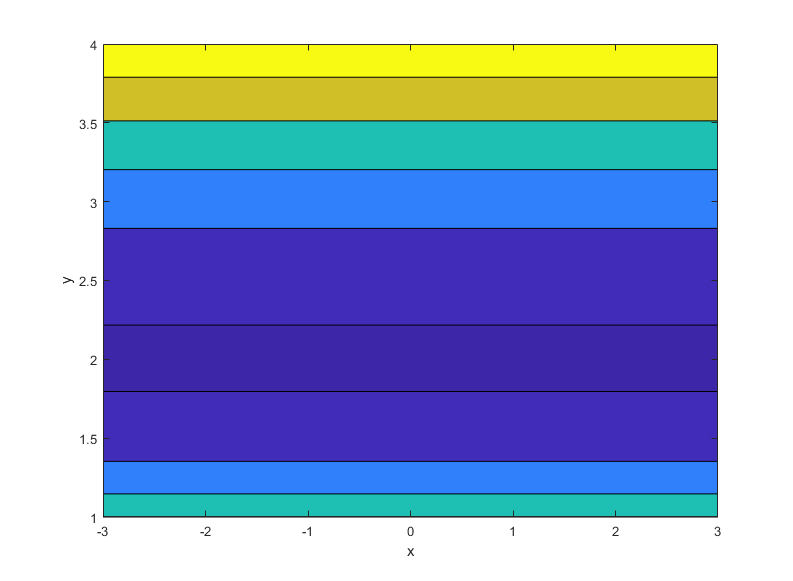
\includegraphics[width = 0.8 \textwidth]{../img/counter.png}
  \caption{Above $y = 2$ we have the compression region and below we have the compression region. As we get to the extremes of our region the lines get closer together, showing the density increasing and vice verse in the region surrounding $y =2$.}
\end{figure}
\end{document}